%!TEX root = ../main.tex

\section{Technische Details}
    \begin{frame}
      \frametitle{Kosten}
      \begin{itemize}
        \item 
          Kosten laut Verband der deutschen Internetwirtschaft, 205 Millionen Euro Investition, min. 50 Millionen pro Jahr, Appendix \cite{kostenVDS}
        \item
          Private E-Mail Provider sowie Anonyme E-Mail Provider nicht betroffen
        \item 
          Provider bis '1000  Teilnehmern' ausgeschlossen, Appendix \cite{emailAusnahme}
      \end{itemize}
    \end{frame}

  \begin{frame}
    \frametitle{Technik IPv4}
    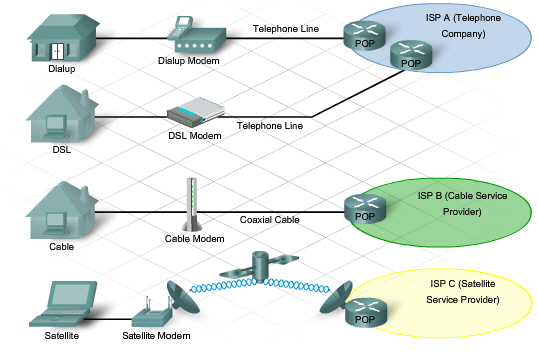
\includegraphics[scale=0.65 ]{sections/img/internet_ipv4.jpg}
  \end{frame}

  \begin{frame}
    \frametitle{Technik IPv6}
    \begin{itemize}
      \item Speicherung der dynamischen Mappings von IPv4 Adressen obsolet
      \item Moeglichkeit jedem Ger"at eine statische Adresse zu zuordnen
      \item \( 16.777.216 \) Adressen in IPv4 \( /24 \), entspricht \( /104 \) in IPv6
      \item IPv6 {\em Privacy Extension} f"ugt Zufall in die Adressen ein zur Verhinderung statischer Adressen f"ur ein Ger"at, Appendix \cite{RFC4941}
    \end{itemize}
  \end{frame}